\chapter{Evaluierung Permissioned Blockchains für B2B}
\label{cha:b2b-eval}

Die Blockchain-Technologie bringt diverse Probleme mit sich, welche je nach Anwendungszweck und Blockchaintyp verschieden große Auswirkungen haben. Für den B2B-Bereich gilt es vor allem die Skalierbarkeit sowie Konsensmechanismen zu analysieren.


\section{Skalierbarkeit}
\label{sec:scalability-eval}
Das CAP-Theorem besagt, dass es in einem verteilten System nur möglich ist, 2 von den 3 folgenden Eigenschaften zu erfüllen: Konsistenz, Verfügbarkeit und Ausfalltoleranz. Bei der Blockchain wären dies: Dezentralisierung, Skalierbarkeit und Nichtangreifbarkeit \cite{SchererPerformanceScalabilityBlockchain2017}. Im Bezug auf die Skalierbarkeit wird vor allem auf den Transaktionsdurchsatz sowie die Bestätigungszeiten von Transaktionen eingegangen. Dazu erfolgt zunächst eine Analyse an aktuellen Public Blockchains, und letztendlich an Permissioned Blockchains. Die Ergebnisse werden ebenfalls auf das CAP-Theorem angewandt. 

\subsection{Public Blockchains}
%TODO: Transaktionsgebühren erwähnen ?
Das Bitcoin-Netzwerk erreicht aktuell einen maximalen Transaktionsdurchsatz von 7 Transaktionen (Unterschiedlich je nach Größe der Transaktionen) pro Sekunde (TPS), bei einer Blockgröße von 1MB.  Hingegen erreicht Paypal 115 TPS, und Visa 2000 TPS (Siehe auch Abb. \ref{fig:tps-comparison}) \cite{ScalabilityBitcoinWiki}. Hinzu kommt, dass ungefähr 170000 unbestätigte Transaktionen\footnote{Unbestätigte Transaktion: Eine Transaktion, welche noch nicht in einen Block vorkommt \cite{AntonopoulosMasteringbitcoin2015}} bestehen \cite{BlockchainFirmaBlockchainChartsUnbestatigte}. Berechnungen von Scherer zeigen, dass bei 11,8 Millionen Nutzern im Bitcoin-Netzwerk, sowie einem Transaktionsdurchsatz von 4 TPS, jeder Nutzer nur nur ca. 10 Transaktionen im Jahr senden kann \cite{SchererPerformanceScalabilityBlockchain2017}. Es ist also ersichtlich, dass Bitcoin nicht skaliert. 

Der Transaktionsdurchsatz ist durch verschiedene Faktoren limitiert. Hauptsächlich durch die limitierte Blockgröße von 1MB, und dem Proof-of-Work: Nur eine bestimmte Anzahl an Transaktionen passt in einen Block, und nur alle 10 Minuten wird einer erstellt. Es gäbe also die Möglichkeit, die Zeit für den Proof-of-Work zu verringern, indem die Schwierigkeit angepasst wird, oder die Blockgröße zu erhöhen. Es gibt jedoch diverse Nachteile, die dadurch entstehen würden. So würde es länger dauern, bis ein Block beim Propagieren durch das Netzwerk alle Nodes erreicht. Dies wiederum würde zu mehr Forks führen, womit Double-Spending-Attacks wahrscheinlicher werden \cite{SchererPerformanceScalabilityBlockchain2017}.   Ebenfalls könnte man argumentieren, dass die Nodes mehr Rechenleistung verschwenden, da Sie den neuen Block später erhalten. Dies führt ebenfalls dazu, dass diese Nodes beim Finden des Proof-of-Work im Nachteil sind, da sie erst später damit beginnen können \cite{BitcoinWikiBlocksizelimit}. Bezüglich der Verringerung der Schwierigkeit um den Proof-of-Work schneller zu erbringen, ...




%===== Ethereum =====

\begin{figure}[htb]
    \centering
      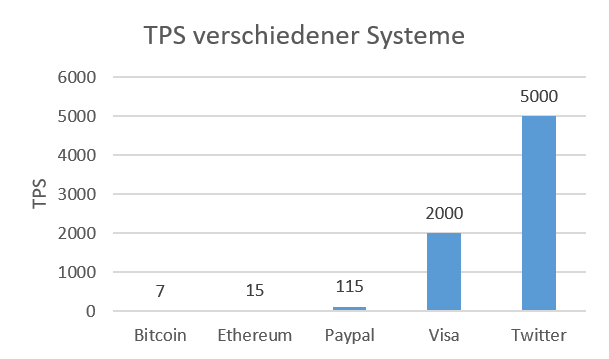
\includegraphics[width=0.95\textwidth,angle=0]{images/tps-comparison}
       \caption{Transaktionsdurchsatz - Vergleich verschiedener Systeme \cite{ScalabilityBitcoinWiki}.}
      \label{fig:tps-comparison}
\end{figure}          



\subsection{Permissioned Blockchains}

%TODO: S.12 ZhengBlockchainChallenges GHOST-Explanation 
%TODO: S.2 SchererPerformance: Less Decentralization --> Better performance and scalability
%TODO: S.3 SchererPerformance: Every node validating every transaction causes bad performance 
%TODO: S.4 SchererPerformance: CAP Theorem --> A distributes system can only guarantee 2 of 3 conditions
%TODO: S.12 SchererPerformance GHOST for better block and transaction times
%TODO: S.19 Scherer: Impact of permissioned Blockchains on Scalability
%TODO: S.19-23 Scherer: Scalability of Bitcoin, Ethereum 15tps
%TODO: S.21 Scherer: Scalability of Fabric
%TODO: S.22 Scherer: Bitcoin PoW Problems
%TODO: S.23 Scherer: "The bottom line is that public networks are not efficient
%TODO: S.20-23 Scherer: CAP Theorem
%TODO: S.23 Scherer: Ethereum is worse off with scaling because of the complexity (Not only money transactions)
%TODO: S.26-28 Scherer: TPS Performance of Fabric
%TODO: S.29-30 Scherer: Scalability Discussion: Throughput with more powerful computers, endorsers, etc.
%TODO: S.31 Scherer: Conclusion is that the question of the fabric performance is not answered
%TODO: S. 1-6 Pongnumkul: Performance ANalysis of Ethereum and Fabric. But how many Participants ? Only private chain ?
%TODO: MinPermissioned: Introduces a concept for better throughput, but it is not tested (??)
%TODO: S.1-6 LiScalable: Introducing a concept with sattelite chains
%TODO: S.2 LiScalable: Blockchain Sharding
%TODO: S.3 Sukhwani: PBFT Performance in Fabric
%TODO: S.23 Scherer: "And since trust is already achieved from outside the network, we do not need much computational"

%TODO: Ethereum All Code executed on every node
%TODO: Erwähnen, wonach sich die Gebühr richtet ?
%TODO: Skalierbarkeit anhand von Bitcoin und Ethereum erklären --> Lösungen betrachten --> Permissioned Blockchains betrachten --> Fazit
%TODO: Dezentralisierung durch weniger Nodes --> Aber Vertrauen durch Identitätsverwaltung gegeben
%TODO: Datenmenge und Redundanz

\begin{itemize}
    \item Transaktionsdurchsatz --> Vor allem wichtig bei IoT-Geräten
    \item Bestätigung von Transaktionen ?
    \item Datenmenge und Redundanz
\end{itemize}

\label{subsec:eval-konsens}
\section{Konsensmechanismen}
%TODO: S.1-4 Gramoli: PoW in Permissioned Chains can be dangerous
%TODO: S.8 ZhengBlockchainChallenges: Consensus Algorithm Byzantine Generals Erklärung
%TODO: S.10-11 ZhengBlockchainChallenges: Consensus Comparison
%TODO: S.4 ZhengBlockchainChallenges: Proof of Stake --> Rich get richer
%TODO: S.7 WustYouNeed: PBFT Consensus is enough for permissioned blockchains
%TODO: S.117 CromanScaling: PBFT could be enough for permissioned blockchains
%TODO: S.22 Scherer: Bitcoin PoW Problems
%TODO: S.3 BenHamida Consensus Algorithms Proof of Elapsed Time, Voting Consensus, PBFT, FBA, Terndermint, Diversity Mining
%TODO: S.6 Consensus Zusammenschluss von Minern/Votern etc.
%TODO: S.3-4 Cachin: Theorie eines Konsensmechanismus
%TODO: S.10-24 Cachin: Consens Algorithms
%TODO: S.1-11 PBFT vs PoA: PBFT is better, because...
%TODO: S.2 SankarSurvery: Stellar Consensuns and PBFT of Hyperledger
%TODO: S.1-14 VukolicQuest: Proof of Work vs BFT


%TODO: Check R3 Consens Algorithm


\begin{itemize}
    \item Nachteile Proof-of-Work
    \item Analyse anderer Konsensmechanismen
\end{itemize}

\section{Privatsphäre}
%TODO: S.4 ZhengBlockchainChallenges: Privacy Leakage and IP Tracking
%TODO: S.1 WustYouNeedBlockchain: Privacy in permissionless chains (zerocash)
%TODO: S.2 WustYouNeedBlockchain: Tensio between Transparency and Privacy

\begin{itemize}
    \item Müssen alle Daten öffentlich verfügbar sein ?
    \item Private Transaktionen realisieren
\end{itemize}

\section{Code Execution}
%TODO: S.2 Gramoli R3 constorium with 45 banks (?)
%TODO: S.2-4 Vukolic More Limitations of Permissioned Blockchains (Code execution, Non Determininstic Execution, Execution on all nodes)

\section{Sonstiges}
%TODO: S.6 BenHamida Real-time analysis and reaction on data (?)
%TODO: Sensorwerte usw. Vertrauen (?)
%TODO: Redundanz der Daten --> Weniger Full Nodes --> Weniger Dezentralisierung --> Höhere Wahrscheinlichkeit eines Zusammenschlusses um Rechenpower zu erreichen





